%! Author = clem
%! Date = 29.06.21

% Preamble
\documentclass[11pt]{article}

% Packages
\usepackage{amsmath}
\usepackage[sfdefault]{roboto}
\usepackage[T1]{fontenc}
\usepackage{array, booktabs}
\usepackage[x11names,table]{xcolor}
\usepackage{textcomp}
\usepackage{graphicx}
\usepackage{hyperref}
\usepackage{float}
\usepackage{tikz}
\usepackage[absolute,overlay]{textpos}
\usepackage{contour}
\usepackage{multicol}
\usepackage{titlesec}
\usepackage{pifont}
\usepackage{ragged2e}
\usepackage[geometry]{ifsym}
\usepackage[pscoord]{eso-pic}% The zero point of the coordinate systemis the lower left corner of the page (the default).

% margin
\usepackage[a4paper, total={0.63 \paperwidth, \paperheight}]{geometry}
\addtolength{\topmargin}{0.1\paperheight}

% color
\definecolor{muted_grey}{rgb}{0.5, 0.5, 0.5}
\definecolor{my_pink}{rgb}{0.92, 0.11, 0.475}
\definecolor{light_mint}{rgb}{0.117, 0.9, 0.5686}
\definecolor{dark_mint}{rgb}{0, 0.55, 0.1}
\definecolor{my_aqua}{rgb}{0, 1, 0.982}
\definecolor{grey_backdrop}{rgb}{1, 1, 1}

%\titlespacing*{\section}{0pt}{0ex}{0ex}

\newcommand{\timeline}{\color{my_pink}\makebox[0pt]{\large---}\hskip-0.5pt\vrule width 1pt\hspace{\labelsep}}
\newcommand{\muted}{\color{muted_grey}}
\newcommand{\placetextbox}[3]{% \placetextbox{<horizontal pos>}{<vertical pos>}{<stuff>}
  \setbox0=\hbox{#3}% Put <stuff> in a box
  \AddToShipoutPictureFG*{% Add <stuff> to current page foreground
    \put(\LenToUnit{#1\paperwidth},\LenToUnit{#2\paperheight}){\vtop{{\null}\makebox[0pt][c]{#3}}}%
  }
}

% center elements left, center, right
\newcommand\textline[4][t]{%
  \par\smallskip\noindent\parbox[#1]{0.6\textwidth}{\raggedright#2}%
  \parbox[#1]{0.5\textwidth}{\raggedleft#4}\par\smallskip%
}

% Document
\begin{document}
%
\includegraphics[scale]{/home/clem/Pictures/profile_pic_dummy}

% ######################################################################################

% left side
\begin{tikzpicture}[remember picture, overlay]
\node[anchor=north west, yshift=4pt, xshift=-4pt]
    at (current page.north west)
    {
\includegraphics[height=\paperheight]{cv_side}};
\end{tikzpicture}

% profile pic
\begin{tikzpicture}[remember picture, overlay]
\node[anchor=north west, yshift=-25pt, xshift=15pt]
    at (current page.north west)
    {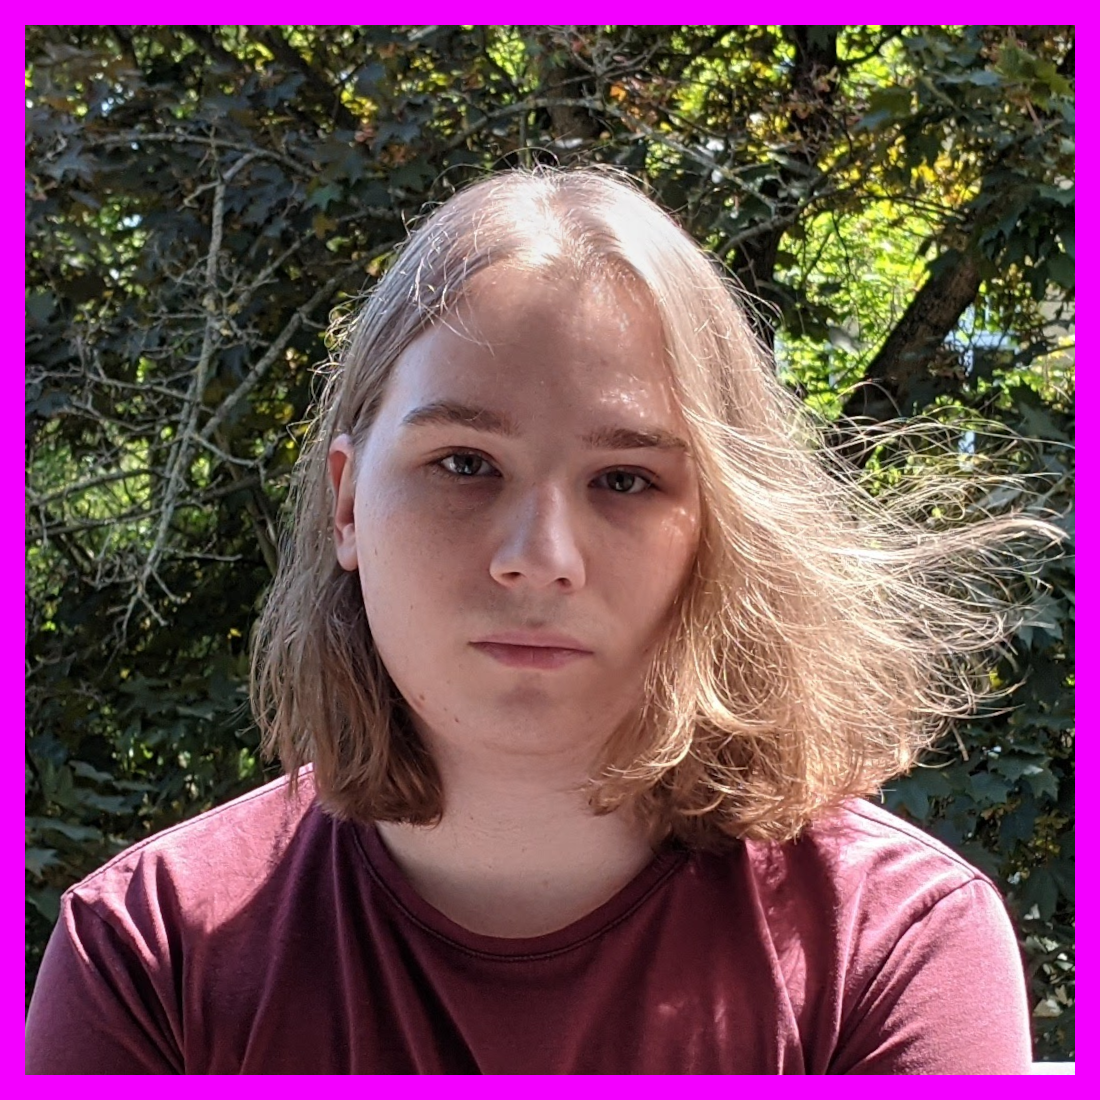
\includegraphics[scale=0.4]{/home/clem/Pictures/profile_pic}};
\end{tikzpicture}

% blurb
\begin{textblock*}{\paperwidth}(24ex, 35pt)
\begin{flushleft}
{\fontsize{30}{35}\selectfont \!Clemens \textbf{Cords}} \newline
{\color{my_pink} {Software Engineer: Visual Computing}} \newline
\newline
\textbf{Mail}: \href{mailto:mail@clemens-cords.com}{mail@clemens-cords.com} \textbf{|} \textbf{Phone}: +49 30 239 438 71 \textbf{|} \href{https://www.linkedin.com/in/clemens-cords/}{\textbf{LinkedIn}} \textbf{|} \href{http://clemens-cords.com/}{\textbf{Blog}} \textbf{|} \href{https://github.com/Clemapfel}{\textbf{GitHub}}
\end{flushleft}
\end{textblock*}

% header
\begin{textblock*}{\paperwidth}(-10pt, 0pt)
\flushright{\color{gray} Juli 2021, Berlin DE}
\end{textblock*}

% timeline
\begin{flushleft}
{\Large \textbf{Work Experience \& Education}}
\end{flushleft}
\begin{tabular}{@{\,}r <{\hskip 2pt} !{\timeline} >{\raggedright\arraybackslash}p{0.6\paperwidth}}
\bottomrule
\addlinespace[1.5ex]
to date \\
2019 & Lead developer at indie video game studio, post-processing and visual fx, engine design, UI/UX; full-time\linebreak\muted(C++ / Lua / GLSL)\linebreak\\
2020 & Graduated FU Berlin with bachelor of science \linebreak
       Thesis developing performance-critical genomic text index \muted(C++)\linebreak\\
2019 & Internship at \href{https://docs.seqan.de/seqan/3-master-user/}{SeqAn3}, developing automated tests and performance benchmarks; 1 Semester part-time \muted(C++)\linebreak\\
2018 & Statistics tutor at FU Berlin; 2 semesters part-time \muted(R)\linebreak\\
2017 & Internship at \href{https://www.roe.berlin/}{radiology practice}, developing image-processing plugin for local MRT / X-Ray imaging server; 2 months full-time \muted(Swift / C++ / Python) \linebreak\\
2015 & Switched to studying bioinformatics, FU Berlin \\
2013 & Studied pure math, TU Berlin \\

\toprule
\end{tabular}

% skills
\begin{flushleft}
\textline{\Large \textbf{Skills}}{}{Proficiency\:}

\textline{\textbf{C++}}{}{\colorbox{grey_backdrop}{5/5\;\;[\,{\color{light_mint} \ding{108}\,\ding{108}\,\ding{108}\,\ding{108}\,\ding{108}}\,]}}
4+ years of experience, including 3 years full-time employment usage.
Knowledge of software design patterns and best-practice operating procedures,
strong foundation in performance-optimization, algorithm-design as well as paralell- and compile-time execution.
Strong belief in keeping code correct, tidy and well-documented at all times {\muted(C++20)}
\textline{\textbf{Lua}}{}{\colorbox{grey_backdrop}{4/5\;\;[\,{\color{light_mint} \ding{108}\,\ding{108}\,\ding{108}\,\ding{108}\,\color{dark_mint}\ding{108}}\,]}}
2 years of experience, high proficency in procedural/functional programming paradigms as well as C-interfacing object-oriented approaches {\muted(Lua 5.4)}\linebreak
\textline{\textbf{GLSL, R}}{}{\colorbox{grey_backdrop}{4/5\;\;[\,{\color{light_mint} \ding{108}\,\ding{108}\,\ding{108}\,\ding{108}\,\color{dark_mint}\ding{108}}\,]}}
\textline{\textbf{Swift, Python, Git}}{}{\colorbox{grey_backdrop}{3/5\;\;[\,{\color{light_mint} \ding{108}\,\ding{108}\,\ding{108}\,\color{dark_mint}\ding{108}\,\ding{108}}\,]}}
%\textline{\textbf{Matlab/Octave, Objective-C, HTML, Doxygen}}{}{\colorbox{grey_backdrop}{2/5\;\;[\,{\color{light_mint} \ding{108}\,\ding{108}\,\color{dark_mint}\ding{108}\,\ding{108}\,\ding{108}\,}]}}
\vspace{1em}
\textbf{German}: fluent at academic level, native tongue \linebreak
\textbf{English}: fluent at academic level \linebreak
\newline
{My game development experience showed me that I do well even in periods of
rapid-pace development under tight deadlines, especially in tight-knit groups.
As part of our engine, I build a font- and text module from scratch and am thus
highly familiar with the nitty-gritty of font-rendering, word processing and
automated text formatting.}%footer
%\vspace{1.5em}
%\flushleft{\footnotesize \color{gray} Please feel free to reach out to me to provide proof or clarification of any details mentioned herein}

\end{flushleft}

\end{document}